% GUIDA VELOCE:
% --------------------------------------------------------------------
% X INIZIA UN UNOVO CAPITOLO:
% \chapter{??? NOME CAPITOLO}}
% 	\section{ ?? }
% 		\subsection{ ?? }
%
% --------------------------------------------------------------------
% PAROLA CONTENUTA NEL GLOSSARIO:
% scrivere la parola seguita da $^g$
% esempio: User$^g$
%
% --------------------------------------------------------------------
% PER ANDARE A CAPO SENZA RIENTRO INSERIRE:
% \\
%
% --------------------------------------------------------------------

% GRASSETO:
% \textbf{parola}
%
% --------------------------------------------------------------------
% CORSIVO:
% \emph{parola}

% --------------------------------------------------------------------
% PER SCRIVERE IN ROSSO:
% \red{parola}
%
% --------------------------------------------------------------------
% PER SCRIVERE TRA VIRGOLETTE
% ''parola''
%
% --------------------------------------------------------------------
% PER EVITARE IL RIENTRO AUTOMATICO DI UN CAPOVERSO:
% \noindent testo....
%
% --------------------------------------------------------------------

% PER SCRIVERE CARATTERI PARTICOLARI COME: { } _  ecc.. SCRIVERLI PRECEDUTI DA \
% ES: \{  \_
%
% --------------------------------------------------------------------
% X INSERIRE UN LINK:
% \url{http://www.math.unipd.it/~tullio/IS-1/2011/Progetto/C3.pdf}
%
% --------------------------------------------------------------------
% PER COMMENTARE INTERE PARTI:
% \comment{ comment }
%
% --------------------------------------------------------------------
% PER SCRIVERE NOTE DURANTE IL TESTO:
% parola \footnote{ note riguardanti la parola }
%
% --------------------------------------------------------------------
% PER SCRIVERE CODICE SORGENTE:
%
% \lstset{language=c++,
% stringstyle=\color{blue}\textrm,
% commentstyle=\rmfamily, numbers= none}

% \begin{lstlisting}
%  CODICE
% \end{lstlisting}
%
% --------------------------------------------------------------------
% !!!!!!!!     PER COSE + COMPLESSE VEDI:     !!!!!!!!!!!!!!!!!!!!!!!
% !!!!!!!!    PMAC/latex/GUIDA LATEX!!!.tex   !!!!!!!!!!!!!!!!!!!!!!!

% per tutto il resto chiedi a lory prima di fare/scrivere cazzate !!!!!!!!!!


\documentclass[10pt,a4paper]{article}

\usepackage[italian]{babel} 
\usepackage[T1]{fontenc} 
\usepackage[utf8x]{inputenc} % uso utf8x xk x linux, mentre latin1 è per windows
\usepackage{lmodern} %insieme di font molto completo consigliato da LatexFacile pg13 in basso
\usepackage{microtype} %migliora riempimento delle righe. vedi LatexImpaziente pg41
%attiva il rientro di ogni prima riga di ogni sezione: capitolo,paragrafo ecc. vd LatexImpaziente pg41
\usepackage{indentfirst}
\usepackage{graphicx} % per inseire immagini
\usepackage[usenames,dvipsnames]{xcolor}
\usepackage{lastpage} %serve per poter scrivere page 1 of N
% setta i bordi della pagina: dx e sx 3.2cm di rientro + nel lato di rilagatura rientra di altri 0mm
\usepackage[a4paper,top=3cm,bottom=3cm,left=3.2cm,right=3.2cm, bindingoffset=0mm]{geometry}
\usepackage{listings} % per inserire codice sorgente
\usepackage{float}  % per gestire oggetti flottanti ( es immagini tabelle posizionebili con "H" che forza il posizionamento nel punto specifico

% serve per creare tabelle lunghe + di una pagina con \begin{longtable} (vd Tabelle.pdf pg11-12)
\usepackage{longtable} 

\usepackage{array} % per mettere b e m nelle creazioni delle tabelle che indicano le dimenzioni delle righe e colonne

\usepackage{fancyhdr} % per impostare lo stile della pagina più personalizzato, + fancyhdr ( per regolare testatina e piè di pagina ) vedi itfancyhrd


\pagestyle{fancy}
% settaggi di pagestyle(fancy)
\lhead{
\includegraphics[scale=0.20]{SevenFold_small}}
%\chead{}
\rhead{\textbf{{%
\NomeDocumento\\ Data: \DataRilascio \\ e-mail: \mail{sevenfold@palomino.it}}}}
\lfoot{\NomeDocumento}
\cfoot{}
\rfoot{ \textbf \thepage\ di \pageref{LastPage}}
\renewcommand{\footrulewidth}{0.4pt}

%ridefinisco il plain per cosare l'indice (a questo punto si potrebbe lasciare tutto il documento in plain
\fancypagestyle{plain}{
\lhead{
\includegraphics[scale=0.20]{SevenFold_small}}
%\chead{}
\rhead{\textbf{{%
\NomeDocumento\\ Data: \DataRilascio \\ e-mail: \mail{sevenfold@palomino.it}}}}
\lfoot{\NomeDocumento}
\cfoot{}
\rfoot{ \textbf \thepage\ di \pageref{LastPage}}
\renewcommand{\footrulewidth}{0.4pt}
}



% da ultimo:
\usepackage{hyperref} %x l'interpretazione di indirizzi o link ipertestuali (vd LatexImpaziente pg47 )
\hypersetup{backref, colorlinks=true, linkcolor=black, urlcolor=black}

\usepackage{url} % x l'interpretazioni di internet o link ipertestuali (vd LatexImpaziente pg47 )
%\UrlFont{color =blue}
%\urlstyle{helvetic}

% Define a new 'leo' style for the package that will use a smaller font.
\makeatletter
\def\url@leostyle{%
  \@ifundefined{selectfont}{\def\UrlFont{\sf}}{\def\UrlFont{\small\ttfamily}}}
\makeatother
%% Now actually use the newly defined style.
\urlstyle{leo}


\newcommand{\mail}[1]{\textcolor{Black}{ \texttt{#1}}} %per interpretare mail (vd LatexImpaziente pg47 )
\newcommand{\cambiaFont}[2]{{\fontencoding{T1}\fontfamily{#1}\selectfont#2}}
\newcommand{\red}[1]{\textcolor{red}{#1}} % per scrivere testo in rosso
\newcommand{\comment}[1]{} % per inserire commenti

% per inserire una nuova lettera nella sezione Glossario
\newcommand{\newLetter}[1]{
\vspace{0.8cm}
\hspace{0.3cm}
\noindent{ \Large{ \textbf{\textcolor{blue}{#1}} } }

\noindent{\color{gray} \line(1,0){415} }\\
%\hspace{0.5cm}
}

\newcommand{\newWord}[1]{\noindent\textbf{\\#1}\\}



% INSERIRE QUI IL NOME DEL DOCUMENTO SEGUITO DA UNO SPAZIO
% ( così il nome si imposta in automatico nelle varie ricorrenze standard)
\newcommand{\NomeDocumento}{Manuale Utente: \emph{Desktop-user }}

% INSERIRE QUI LA DATA DELLA VERSIONE DEL RILASCIO
\newcommand{\DataRilascio}{2012/09/17}

% INSERISCI LA VERSIONE ATTUALE
\newcommand{\VersioneAttuale}{v2.0.0}

% INSERIRE QUI L'ACRONIMO DEL DOCUMENTO. ESEMPIO: Analisi Dei Requisiti = AR
% Quando inserite l'acronimo qui, dovete rinominare i file presenti nella cartella
% del tipo '??-cap1-NomeCapitolo.tex' sostituendo i '??' con l'acronimo scelto!!
\newcommand{\AcronimoDocumento}{??}

\begin{document}


% --------------------------------------------------------------------

% TITOLO ( 1° pagina)

\vspace*{2.5cm}
\begin{center}

%\cambiaFont{Cyklop}{Sevenfold}
%\cambiaFont{fve}{\Huge{Sevenfold}}

\includegraphics[scale=0.35]{SevenFold_big}

\vspace{2cm}

\cambiaFont{fve}{\Huge{\NomeDocumento}}\\
\vspace*{1cm}


\end{center}


% --------------------------------------------------------------------

\vspace*{2cm}
\begin{center}

\begin{tabular}{ r | l }
\multicolumn{2}{c}{\textbf{\huge{Informazioni sul documento}} }\\
\hline
\rule[-1.5mm]{0mm}{0.7cm}
\textbf{Titolo documento} & \NomeDocumento\\
\rule[-1.5mm]{0mm}{0.5cm}
\textbf{Data creazione}& 2012/09/19\\
\rule[-1.5mm]{0mm}{0.5cm}
\textbf{Distribuito da}& Gruppo SevenFold\\
\rule[-1.5mm]{0mm}{0.5cm}
\textbf{Destinato a}&Prof. Ghiraldo Filippo\\
&Gruppo Sevenfold\\

\end{tabular}

\end{center}


% --------------------------------------------------------------------

% SOMMARIO ( 2° pagina)

\newpage

\vspace*{0.5cm} % il vertical space va preceduto da una riga vuota!!!
\begin{center}

\textbf{{\huge{Sommario}}}

\vspace*{0.2cm} % il vertical space va preceduto da una riga vuota!!!

Questo documento ha lo scopo di descrivere il corretto utilizzo dell'applicazione Woty$^g$ inerentemente alle funzionalità del \textit{Desktop-user}.



\end{center}


% --------------------------------------------------------------------



% --------------------------------------------------------------------
% INDICI:

\newpage
% INDICE CAPITOLI
\tableofcontents % genera l'indice di tutto il documento

\let\cleardoublepage\clearpage % toglie la pagina bianca dopo l'indice

% INDICE TABELLE
%\listoftables

% INDICE FIGURE
%\listoffigures


% --------------------------------------------------------------------

% INSERISCO IL I° CAPITOLO ''Introduzione''

\newpage
\section{Introduzione}
	\subsection{Cos'è Woty}
Il sistema Woty consiste in una piattaforma innovativa per l'apprendimento comportamentale nell'ambito della sicurezza sul lavoro, che utilizza le tecniche della gamification per incentivare il coinvolgimento e la partecipazione degli utenti e per scardinare l'instaurarsi di abitudini errate.\\
Questo sistema si prefigge di garantire l'insegnamento della sicurezza sul lavoro agli utenti utilizzatori, attraverso la risoluzione periodica di quest$^g$ specifiche all'ambito aziendali del singolo utente.


\subsection{Utente destinatario del manuale}
Il manuale è destinato agli utenti che utilizzano le applicazioni \textbf{Woty Desktop} e \textbf{Woty Web} attraverso l'utilizzo di una postazione fissa; tali utenti vengono qui denominati ''Desktop-user''.\\
Questi utenti sono dipendenti di un'azienda che avrà scelto di utilizzare la piattaforma Woty, per i quali è stato assegnato loro un account di iscrizione al sistema.


\subsection{Come leggere il manuale}
	
Per ognuna delle due applicazioni a disposizione dell'utente \textbf{Woty Desktop} e \textbf{Woty Web} è presente una specifica guida così strutturata:

\begin{enumerate}
\item \textbf{Woty Desktop}

\begin{enumerate}
\item Requisiti software
\item Installazione o rimozione applicazione
\item Avvio applicazione
\item Significato icone
\item Messaggi visualizzati
\item Opzioni menù
\item Errori possibili
\end{enumerate}



\item \textbf{Woty Web}

\begin{enumerate}
\item Requisiti software
\item Login
\item Menu di navigazione
\item Home
\item Profile
\item Pending Quest
\item List
\item Errori possibili

\end{enumerate}

\end{enumerate}


Tutti i termini e gli acronimi presenti nel seguente documento che necessitano di definizione saranno seguiti da una ''g'' ad apice ( E.g. Woty$^g$ ) alla loro prima occorrenza e saranno riportati con le rispettive spiegazioni al termine del manuale nell'apposita sezione \emph{Glossario} \ref{glossario}.




\subsection{Come riportare problemi e malfunzionamenti}
In caso di malfunzionamenti o errori del sistema, l'utente sarà tenuto a segnalare il problema riscontrato, avvisando il proprio responsabile interno di sistema e dando una descrizione il più dettagliata possibile dell'errore avvenuto.
In particolare sarà necessario comunicare le seguenti informazioni:

\begin{enumerate}
\item data e ora in cui il problema è stato riscontrato
\item descrizione del problema
\item situazione in cui il problema si è verificato
\end{enumerate}


Per qualsiasi altro problema contattare l'indirizzo: \mail{sevenfold@palomino.it}




% ---------------------------------------------------------------------------



\section{Istruzioni per l'uso}



\subsection{Woty desktop}
\label{wd}
Consiste in un'applicazione del tipo tray icon$^g$ utilizzabile attraverso personal computer, che gestisce le notifiche di un utente, avvisandolo della presenza di nuove notifiche.

\subsubsection{Requisiti software}
L'applicazione Woty Desktop può essere installata ed eseguita correttamente negli ambienti Windows, OSX o Ubuntu Linux in base alle seguenti versioni:

\begin{itemize}
\item \textbf{Windows}:
	\begin{itemize}
	\item Microsoft Windows XP
	\item Microsoft Windows Vista
	\item Microsoft Windows 7
	\end{itemize}

\item \textbf{OSX}:
	\begin{itemize}
	\item Apple MacOs 10.5, 10.6, 10.7
	\item Per poter visualizzare i messaggi di notifica è necessario aver installato l'applicazione \textit{Growl} scaricabile alla pagina \url{http://growl.info/downloads}
	\end{itemize}

\item \textbf{Ubuntu Linux}:
	\begin{itemize}
	\item Ubuntu Linux versioni 10.04, 10.11, 11.04, 11.11. Il funzionamento su altre distribuzioni GNU/Linux è possibile ma non garantito.
	\end{itemize}


\end{itemize}




\subsubsection{Installazione o rimozione applicazione}
L'applicazione Woty Desktop potrà essere scaricata gratuitamente selezionando il proprio sistema operativo$^g$ dalla home page all'indirizzo \url{http://178.255.240.201/home}.
Successivamente installare l'applicazione seguendo la procedura guidata.


In base al sistema operativo utilizzato seguire la rispettiva procedura di disinstallazione:

\begin{itemize}
\item Windows:\\
Avviare il gestore delle applicazioni, selezionare Woty e cliccare su ''disinstalla''

\item OsX:\\
Accedere al Finder, aprire la cartella applicazioni, quindi selezionare Woty ed eliminarla

\item Ubuntu Linux:\\
Aprire il terminale e digitare il comando: \textit{sudo apt-get remove woty}

\end{itemize}




\subsubsection{Avvio applicazione}
Dopo aver installato Woty Desktop, eseguire l'applicazione:
al suo avvio comparirà un messaggio di notifica che indicherà il corretto funzionamento e avviserà l'utente di effettuare l'autenticazione alla piattaforma Woty, inoltre nell'area system tray$^g$ della traybar$^g$ del proprio sistema operativo comparirà un'icona tray icon$^g$  dell'applicazione Woty desktop, come illustrato in figura \ref{wd-trayicon}.

\begin{center}
\begin{figure}[ht]
\centering
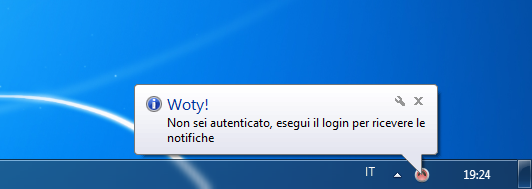
\includegraphics[scale=0.6]{images/wotyDesktop/schreenshots/msg-start.png}
\caption{Woty Desktop - Tray Icon}
\label{wd-trayicon}
\end{figure}
\end{center}


	\subsubsection{Significato icone}
L'icona tray icon che verrà visualizzata, potrà essere di 4 differenti tipi come illustrato in figura \ref{wd-icone}.

\begin{center}
\begin{figure}[H]
\centering
\begin{tabular}{ m{1.5cm} m{1.5cm} m{1.5cm} m{1.5cm} }
\hline
\multicolumn{4}{c}{ Descrizione icone}\\
\hline
\multicolumn{4}{r}{ \vspace*{0.5cm} }\\

\includegraphics[scale=0.14]{images/wotyDesktop/icons/ico3.png} & 

\includegraphics[scale=0.14]{images/wotyDesktop/icons/ico2.png} & 

\includegraphics[scale=0.14]{images/wotyDesktop/icons/ico1.png} &

\includegraphics[scale=0.14]{images/wotyDesktop/icons/ico0.png} \\
\multicolumn{4}{r}{ \vspace*{0.2cm} }\\
Icona (1) & Icona (2) & Icona (3) & Icona (4) \\
\multicolumn{4}{r}{ \vspace*{0.2cm} }\\
\end{tabular}
\caption{Woty Desktop - Icone}
\label{wd-icone}
\end{figure}
\end{center}



\begin{itemize}


\item L'icona (1) indica lo stato di non autenticazione, non è stato eseguito il login al sistema Woty e non vengono ricevute le notifiche.

\item L'icona (2) indica lo stato off-line, il computer non è connesso alla rete internet.

\item L'icona (3) indica lo stato di autenticazione, è stato eseguito il login al sistema Woty e non sono presenti notifiche per l'utente.

\item L'icona (4) indica lo stato di autenticazione, è stato eseguito il login al sistema Woty e sono presenti delle notifiche riguardanti l'utente.
\end{itemize}

\subsubsection{Messaggi visualizzati}
L'utente potrà visualizzare diversi tipi di messaggi a seconda del verificarsi di diversi eventi.
Di seguito sono illustrati i possibili messaggi che l'utente potrà visualizzare.


\begin{itemize}
\item Messaggio di avvio dell'applicazione nello stato di non autenticazione:

\begin{center}
\begin{figure}[H]
\centering
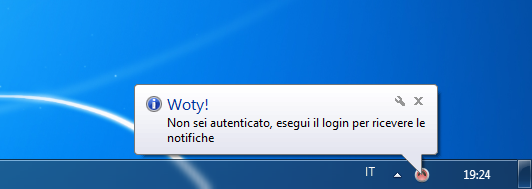
\includegraphics[scale=0.64]{images/wotyDesktop/schreenshots/msg-start.png}
\caption{Woty Desktop - Messaggio di non autenticazione}
\label{wd}
\end{figure}
\end{center}

\item Messaggio di mancata connessione alla rete internet:

\begin{center}
\begin{figure}[H]
\centering
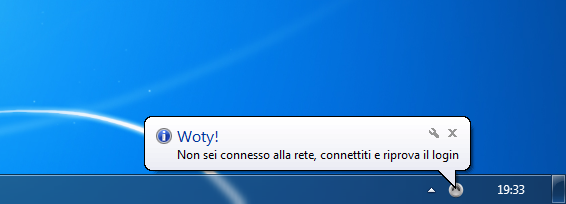
\includegraphics[scale=0.6]{images/wotyDesktop/schreenshots/msg-offline.png}
\caption{Woty Desktop - Messaggio di non connessione alla rete}
\label{wd}
\end{figure}
\end{center}


\item Messaggio di login avvenuto con successo: 

\begin{center}
\begin{figure}[H]
\centering
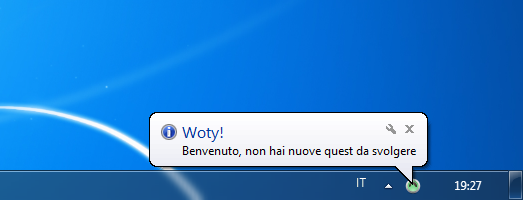
\includegraphics[scale=0.6]{images/wotyDesktop/schreenshots/msg-login.png}
\caption{Woty Desktop - Messaggio di login}
\label{wd}
\end{figure}
\end{center}


\item Messaggio di logout avvenuto con successo: 

\begin{center}
\begin{figure}[H]
\centering
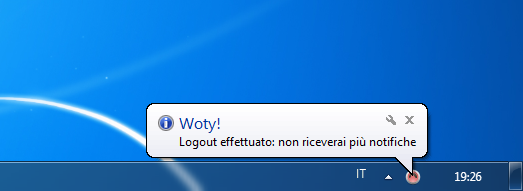
\includegraphics[scale=0.6]{images/wotyDesktop/schreenshots/msg-logout.png}
\caption{Woty Desktop - Messaggio di logout}
\label{wd}
\end{figure}
\end{center}


\item Messaggio di notifica: 

\begin{center}
\begin{figure}[H]
\centering
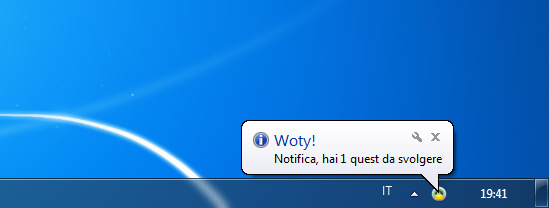
\includegraphics[scale=0.6]{images/wotyDesktop/schreenshots/msg-notify.png}
\caption{Woty Desktop - Messaggio di notifiche}
\label{wd}
\end{figure}
\end{center}

\end{itemize}


\subsubsection{Opzioni menù}
Per visualizzare il menù fare click nell'icona di Woty Desktop, comparirà il menù come illustrato in figura \ref{wd-menu}.

\begin{center}
\begin{figure}[H]
\centering
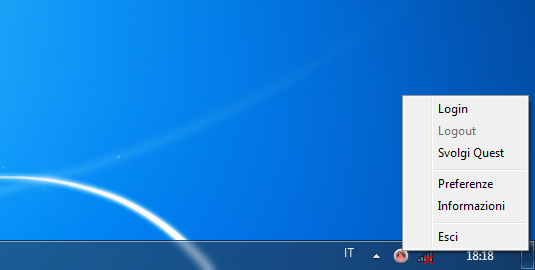
\includegraphics[scale=0.6]{images/wotyDesktop/schreenshots/menu.png}
\caption{Woty Desktop - Menù}
\label{wd-menu}
\end{figure}
\end{center}

Per ognuna delle opzioni indicate nel menù, di seguito ne verrà riportata una illustrazione:

\begin{itemize}
\item \textbf{Login}:
questa funzione del menu permette di effettuare l'autenticazione alla piattaforma Woty e, al suo click, comparirà una form per l'inserimento delle credenziali di accesso quali email e password, come illustrato in figura \ref{wd-login}.

\begin{center}
\begin{figure}[H]
\centering
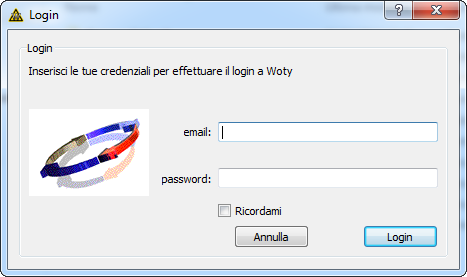
\includegraphics[scale=0.7]{images/wotyDesktop/schreenshots/window-login.png}
\caption{Woty desktop - Login}
\label{wd-login}
\end{figure}
\end{center}

Nel campo \textbf{email} dovrà essere inserita l'email dell'utente e nel campo \textbf{password} la password, inoltre spuntando il campo \textbf{Ricordami} sarà possibile scegliere se mantenere memorizzata l'autenticazione così da non dover inserire le credenziali ad ogni successivo avvio del programma.

\ \
\item \textbf{Logout}:
Permette di effettuare il logout dell'utente dal sistema Woty. Tutte le informazioni riguardanti le credenziali di accesso dell'utente verranno cancellate.


\ \
\item \textbf{Svolgi quest}:
Permette all'utente l'accesso diretto alla sezione quest$^g$ della piattaforma Woty tramite browser. Potrebbe essere richiesto di eseguire il login anche nell'applicazione Woty Web nel caso in cui l'utente non sia già loggato.

\ \
\item \textbf{Preferenze}:
Permette all'utente di impostare la lingua dell'applicazione.

\begin{center}
\begin{figure}[H]
\centering
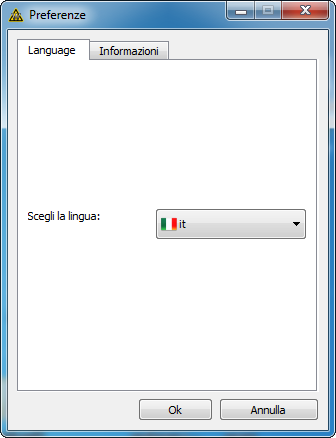
\includegraphics[scale=0.68]{images/wotyDesktop/schreenshots/window-preferences.png}
\caption{Woty desktop - Preferenze}
\label{wd-preference}
\end{figure}
\end{center}


\ \
\item \textbf{Informazioni}:
Permette all'utente di visualizzare informazioni sull'applicazione.
Da qui è possibile inoltre accedere alla pagina internet del sistema Wory attraverso il link \underline{\textit{Ulteriori informazioni su Woty}}


\begin{center}
\begin{figure}[H]
\centering
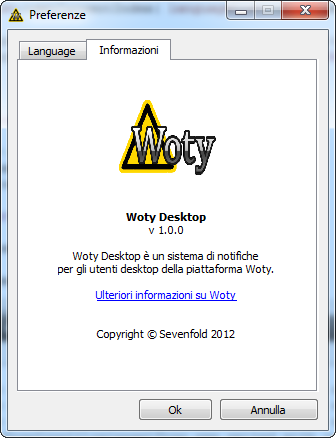
\includegraphics[scale=0.7]{images/wotyDesktop/schreenshots/about.png}
\caption{Woty desktop - Informazioni}
\label{wd-informazioni}
\end{figure}
\end{center}



\ \
\item \textbf{Esci}:
Permette all'utente la chiusura dell'applicazione.


\end{itemize}





\subsubsection{Errori possibili}
Per qualsiasi tipo di errore, fare riferimento alla sezione \emph{''Come riportare problemi e malfunzionamenti''}.


\newpage
\subsection{Woty web}
\label{ww}
Consiste nell'applicazione web, accessibile tramite un normale browser (possibilmente aggiornato alle versioni più recenti) all'indirizzo \url{http://178.255.240.201}, dalla quale un utente potrà accedere a tutte le funzionalità a lui disponibili.


\subsubsection{Requisiti software}
L'applicazione Woty Web può essere utilizzata correttamente secondo le seguenti dipendenze dai browser nelle loro versioni minime necessarie. Non potrà essere garantito un corretto funzionamento dell'applicazione nel caso di utilizzo di versioni browser inferiori rispetto a quelle riportate.

\begin{itemize}
\item Microsoft Internet Explorer 8.0+
\item Apple Safari 5.0.0+
\item Firefox 4.0+
\item Google Chrome 16.0+
\end{itemize}


\subsubsection{Login}
E' possibile effettuare il login all'applicazione accedendo alla home page dell'applicazione WotyWeb all'indirizzo \url{http://178.255.240.201} e premendo nella sezione \textbf{Login} presente nel menu di navigazione. Successivamente inserire le proprie credenziali di accesso email e password negli appositi campi della form, come illustrato nella figura \ref{ww-login}.

\begin{center}
\begin{figure}[H]
\centering
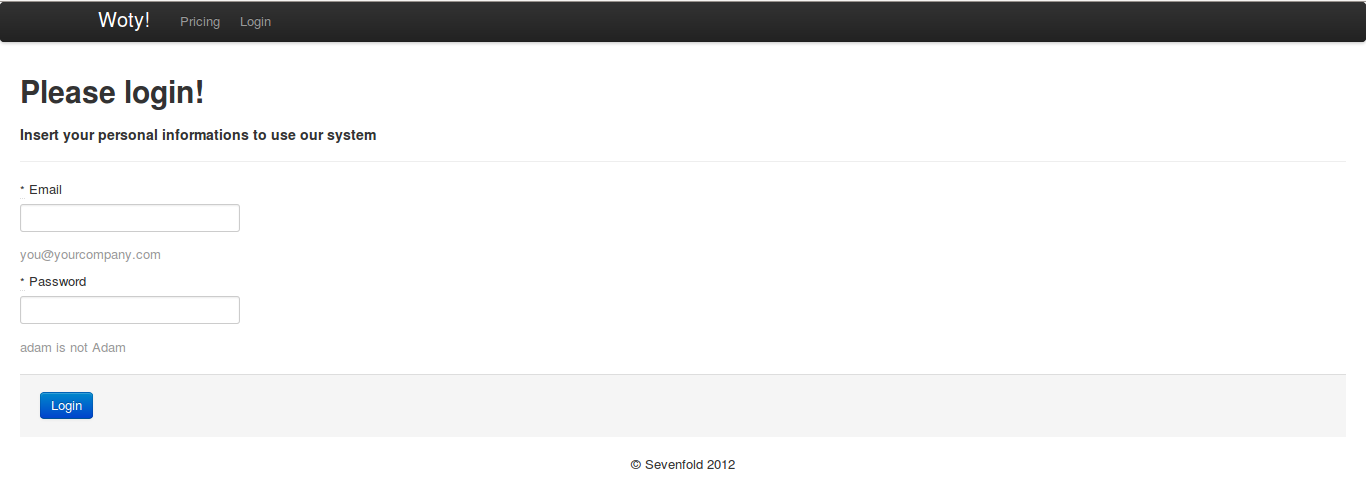
\includegraphics[scale=0.35]{images/wotyWeb/login.png}
\caption{Woty Web - Login}
\label{ww-login}
\end{figure}
\end{center}



\subsubsection{Menu di navigazione}
E' possibile navigare tra le pagine dell'applicazione attraverso il menu di navigazione presente in ogni pagina nella barra superiore, come illustrato in figura \ref{ww-menu}.

\begin{center}
\begin{figure}[H]
\centering

\includegraphics[scale=0.35]{images/wotyWeb/menu.png}
\caption{Woty Web - Menu di navigazione}
\label{ww-menu}
\end{figure}
\end{center}


Descrizione delle sezioni del menu:
\begin{itemize}
\item \textbf{Home}:\\
Sezione che permette la visualizzazione di stream di eventi e informazioni sulle classifiche del proprio workgroup

\item \textbf{Profile}:\\
Sezione che permette di visualizzare e modificare le proprie informazioni personali

\item \textbf{Pending Quest}:\\
Sezione indicante le Quest in sospeso da svolgere

\item \textbf{List}:\\
Sezione che permette la visualizzazione dell'indice completo dell'item selezionato, quale ad esempio Quest, User, Customer, etc.

\item \textbf{Logout}:\\
Permette di effettuare il logout dall'applicazione Woty
\end{itemize}


\subsubsection{Home}
Attraverso la sezione \textbf{Home} è possibile accedere alla pagina degli stream del proprio workgroup come illustrato in figura \ref{ww-home}.


\begin{center}
\begin{figure}[H]
\centering
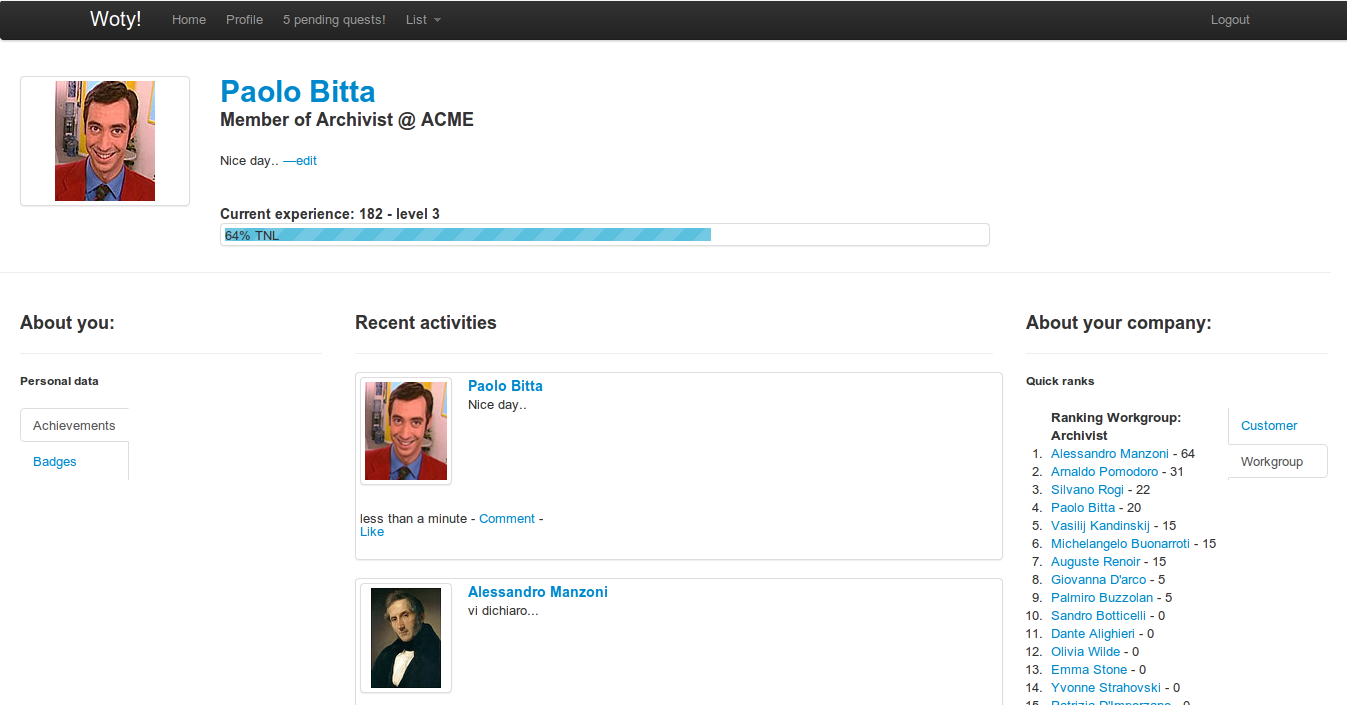
\includegraphics[scale=0.35]{images/wotyWeb/home.png}
\caption{Woty Web - Home}
\label{ww-home}
\end{figure}
\end{center}


\textbf{Edit}:\\
Link che permette di modificare il proprio stato inserendo una frase preferita che sarà visualizzata dagli altri utenti appartenenti al proprio customer.\\


\textbf{Current experience}:\\
Barra nella quale vengono visualizzati i punti esperienza acquisiti nel tempo dall'utente attraverso lo svolgimento corretto di quest.\\

\textbf{About you}:\\
Area riservata alla visualizzazione dei badge$^g$ e achievement$^g$ raggiunti dallo specifico utente attraverso la risoluzione corretta di quest.\\

\textbf{Recent activities}:\\
Area riservata per la visualizzazione di stream di eventi riguardanti le azioni recenti svolte dagli altri user appartenenti allo stesso Workgroup di lavoro; in questo modo ogni utente potrà essere sempre aggiornato in tempo reale a riguardo degli altri utenti.\\


\textbf{About your company}:\\
Area riservata per la visualizzazione di informazioni riguardanti il proprio Customer di appartenenza. 




\subsubsection{Profile}
Attraverso la sezione \textbf{Profile} è possibile accedere alla pagina del proprio profilo personale come illustrato in figura \ref{ww-profile}.


\begin{center}
\begin{figure}[H]
\centering
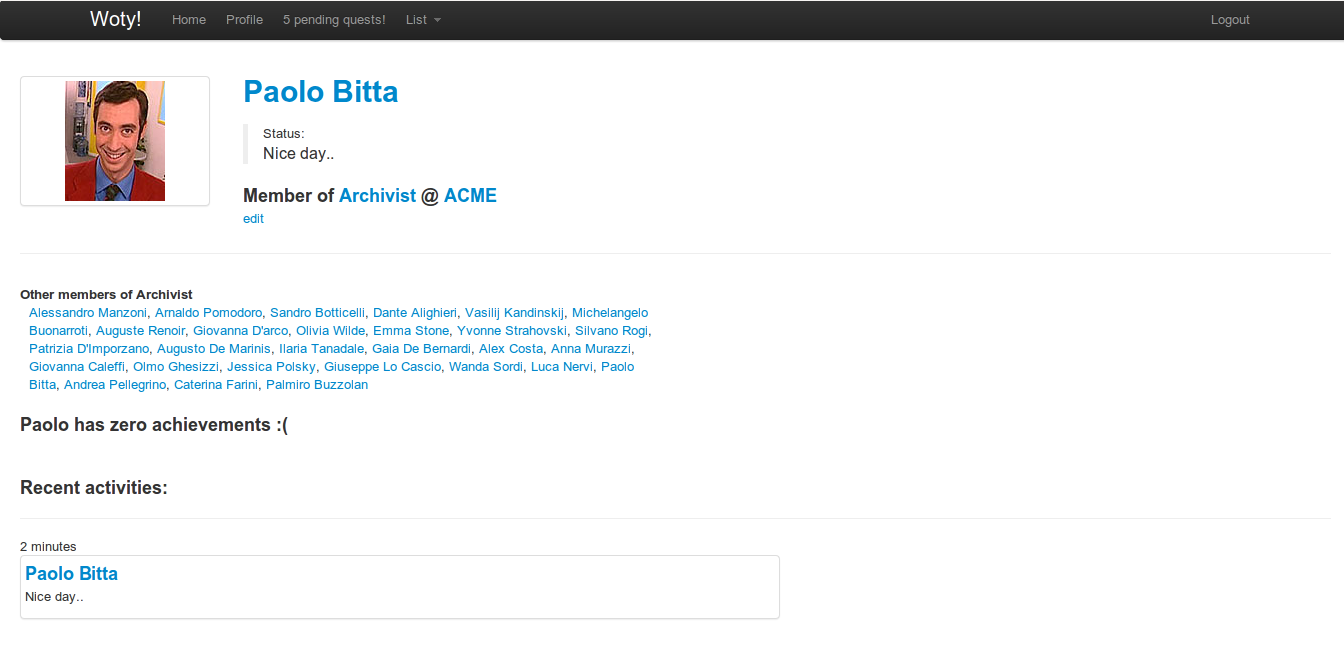
\includegraphics[scale=0.35]{images/wotyWeb/profile.png}
\caption{Woty Web - Profile}
\label{ww-profile}
\end{figure}
\end{center}

\textbf{Edit}:\\
Link che permette di modificare le proprie informazioni personali.\\






\subsubsection{Pending Quest}
Attraverso la sezione \textbf{ Pending Quest }, se l'utente non ha quest in sospeso può richiederne l'assegnazione, altrimenti verrà indirizzato alla pagina per la visualizzazione delle quest, come illustrato in figura \ref{ww-doQuest}.


\begin{center}
\begin{figure}[H]
\centering
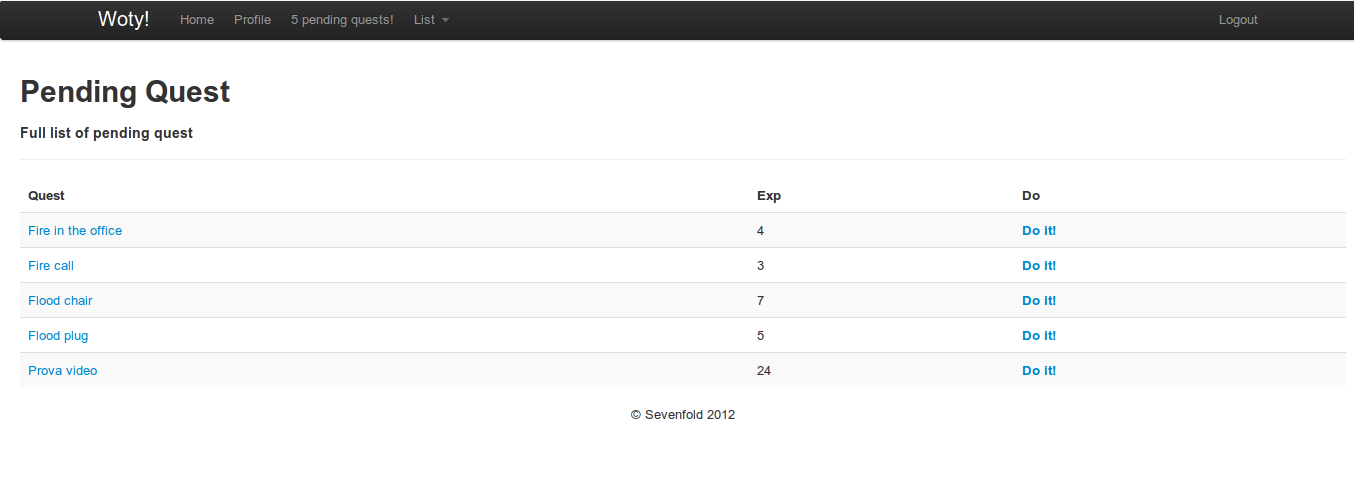
\includegraphics[scale=0.35]{images/wotyWeb/doQuest.png}
\caption{Woty Web - Svolgi Quest}
\label{ww-doQuest}
\end{figure}
\end{center}



Da qui è possibile visualizzare la quest cliccando nel nome della quest, oppure è possibile svolgere la quest attraverso il link \textbf{Do it!}.
Di seguito viene riportato un esempio di una Quest da svolgere:

\begin{center}
\begin{figure}[H]
\centering
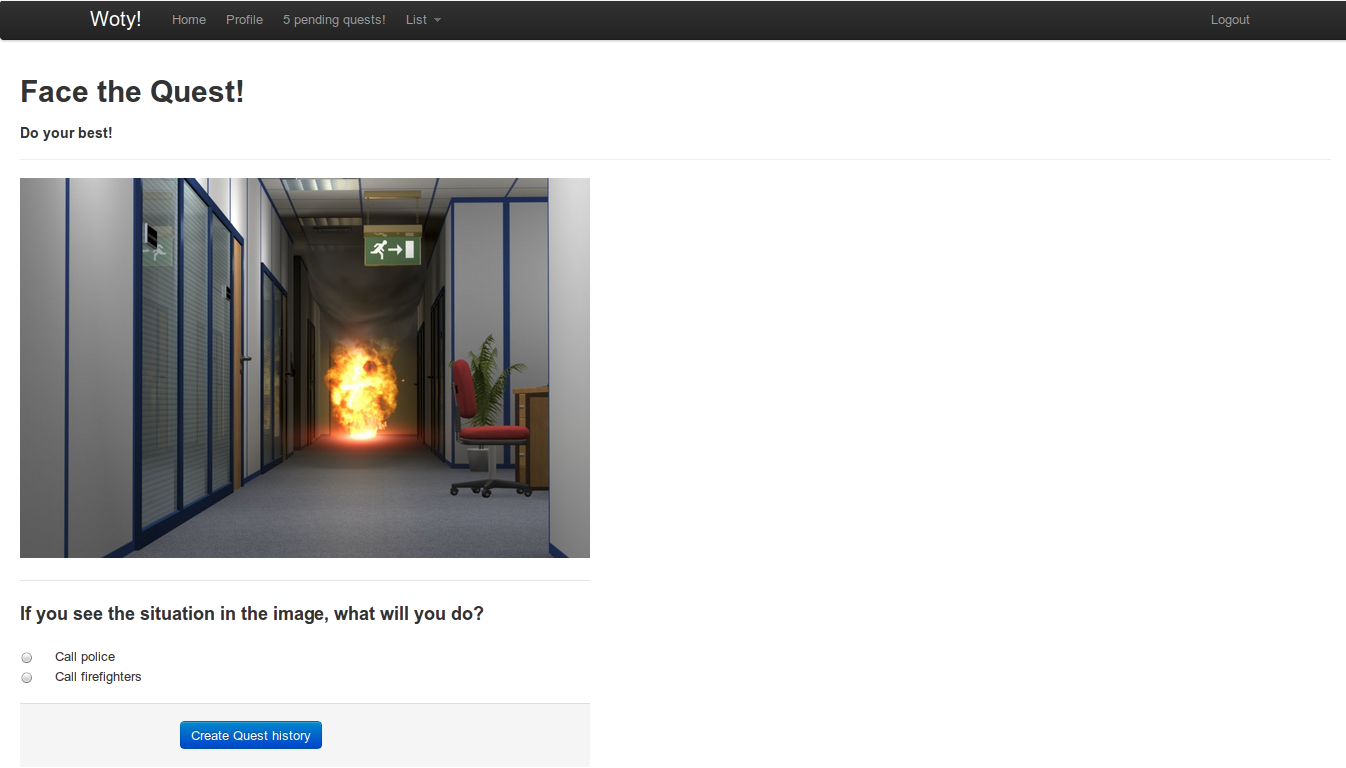
\includegraphics[scale=0.35]{images/wotyWeb/quest.png}
\caption{Woty Web - Svolgi Quest}
\label{ww-quest}
\end{figure}
\end{center}


 Attraverso un corretto svolgimento delle quest l'utente acquisirà punti esperienza e potrà raggiungere nuovi badge e achievement incrementando la propria posizione nella classifica.



\subsubsection{List}
Attraverso la sezione \textbf{List} è possibile visualizzare per ogni item selezionato l'indice completo. E' possibile visualizzare l'indice per i seguenti item:

\begin{itemize}
\item[-] \textbf{Achievement}\\
Consiste nell'indice degli achievement che gli utenti possono raggiungere

\item[-] \textbf{Customer}\\
Consiste nell'indice dei customer iscritti al sistema Woty

\item[-] \textbf{Quest}\\
Consiste nell'indice di quest create

\item[-] \textbf{Plan}\\
Consiste nell'indice dei piani tariffari creati per i customer

\item[-] \textbf{User}\\
Consiste nell'indice degli utenti di ogni customer iscritti al sistema woty

\item[-] \textbf{Workgroup}\\
Consiste nell'indice dei gruppi di lavoro necessari per suddividere gli utenti all'interno di un customer


\end{itemize}




\subsubsection{Errori possibili}
Per qualsiasi tipo di errore, fare riferimento alla sezione \emph{''Come riportare problemi e malfunzionamenti''}.


% ---------------------------------------------------------------------------

\newpage

\section{Appendice}


\subsection{Messaggi di errore e loro significato}

Per l'applicazione Woty Server i principali messaggi di errore che possono essere visualizzati sono:
\begin{itemize}
\item \textbf{Invalid email or password}\\
Messaggio indicante che le credenziali d'accesso inserite nella form di login non sono corrette

\item \textbf{You are not authorized to access this page}\\
Messaggio indicante un tentativo di accesso non autorizzato ad una pagina cercata dall'utente

\item \textbf{Routing Error}\\
Messaggio indicante che la pagina cercata non è stata trovata o è inesistente
\end{itemize}


\ \
\subsection{Glossario}

\label{glossario}


\newLetter{A}
\newWord{Achievement}
Gratifica all'utente, ottenuto in seguito al raggiungimento di determinati obiettivi.



\newLetter{B}
\newWord{Budget}
Dall'inglese ''distintivo'', è un premio virtuale garantito ad un utente per aver completato
un'azione all'interno di vincoli prestabiliti.



\newLetter{Q}
\newWord{Quest}
Una quest è una una sfida che l'User dovrà compiere.


\newLetter{S}
\newWord{Sistema Operativo}
E' un particolare software, installato su un sistema di elaborazione, che funge da ''base'' al quale si appoggiano gli altri software, che dunque dovranno essere progettati in modo da essere riconosciuti e supportati da quel particolare sistema operativo.

\newWord{System Tray}
E' una sezione della Taskbar, generalmente utilizzata per visualizzare l'orologio e le icone di alcuni programmi così da permettere all'utente di poterli costantemente visualizzare e cliccarli.



\newpage


\newLetter{T}
\newWord{Taskbar}
Consiste in una barra che viene visualizzata sul desktop di un computer e viene utilizzata per avviare e monitorare le applicazioni in esecuzione.

\newWord{Tray Icon}
Consiste in una singola icona presente nell'area System Tray che indica uno specifico programma attivo in background. 


\newLetter{W}
\newWord{Woty}
acronimo dal doppio significato WOrk safeTY, oppure Worker Of The Year.


\end{document}
